\newpage
\section{Aufgabe 2}
In dieser Aufgabe soll die Schallgeschwindigkeit und der Isentropenindex bzw. Adiabatenkoeffizient über die Resonanzfrequenzen in einem Rohr bestimmt werden. Dabei ist das Rohr in einem Fall offen und im anderen geschlossen.
\subsection{Aufbau}
Vorhanden ist ein Rohr, dass auf der einen Seite einen Lautsprecher und auf der anderen Seite eine Öffnung hat, die man jedoch mit einem Brettchen verschließen kann. Der Lautsprecher wird mit Bananensteckerkabeln mit dem Funktionsgenerator verbunden um bestimmte Schallwellen im Rohr zu erzeugen. Gemessen wird qualitativ die Lautstärke an einer kleinen Öffnung am Rohr indem ein Mikrophon an ein Wechselspannungsmessgerät angeschlossen wird.
\subsection{Durchführung}
Es werden sinusförmige Wechselströme auf den Lautsprecher gegeben und die Frequenz am Funktionsgenerator so Eingestellt, dass ein Maximum der Lautstärke gemessen wird.
\subsection{Fehlerabschätzung}
Leider ist die Messung der Frequenz sehr ungenau, da weder der Funktionsgenerator eine genaue Frequenz anzeigt, noch die Frequenz sehr exakt eingestellt werden konnte, da die Lautstärke in einem gewissen Bereich eher Konstant war. Der Fehler der Frequenz wird geschätzt auf:
\begin{equation}
\Delta f = 7\% \notag
\end{equation}
\newpage
\subsection{Messwerte}
Ermittelt wurden folgende Werte für Resonanzfrequenzen:

\begin{center}
\begin{tabular}{c|cc}
\multirow{2}{*}{Ordung \(n\)} & \multicolumn{2}{c}{Resonanzfrequnzen \(f\)}\\
 & Messreihe 1 & Messreihe 2 \\\hline
\(1\) & \(73\) & \(75\) \\ 
\(2\) & \(227\) & \(217\) \\ 
\(3\) & \(416\) & \(457\) \\ 
\(4\) & \(620\) & \(616\) \\ 
\(5\) & \(782\) & \(786\) \\ 
\(6\) & \(958\) & \(955\) \\ 
\(7\) & \(1114\) & \(1123\) \\ 
\(8\) & \(1286\) & \(1292\) \\ 
\(9\) & \(1415\) & \(1420\) \\ 
\(10\) & \(1573\) & \(1580\) \\ 
\(11\) & \(1730\) & \(1730\) \\ 
\(12\) & \(1887\) & \(1883\) \\ 
\(13\) & \(2068\) & \(2064\) \\
\end{tabular}
\captionof{table}{Messwerte der geschlossenen Röhre}
\vspace{1cm}
\begin{tabular}{c|c}
Ordnung \(n\) & Resonanzfrequnzen \(f\) \\\hline
\(1\) & \(60\) \\ 
\(2\) & \(153\) \\ 
\(3\) & \(278\) \\ 
\(4\) & \(350\) \\ 
\(5\) & \(395\) \\ 
\(6\) & \(528\) \\ 
\(7\) & \(683\) \\ 
\(8\) & \(866\) \\ 
\(9\) & \(1030\) \\ 
\(10\) & \(1205\) \\ 
\(11\) & \(1471\) \\ 
\(12\) & \(1636\) \\ 
\(13\) & \(1784\) \\ 
\(14\) & \(1955\) \\ 
\(15\) & \(2243\) \\
\end{tabular}
\captionof{table}{Messwerte der offenen Röhre}
\end{center}
Die Länge der Röhre \(l\) wurde aus dem Platzskript entnommen:
\begin{align}
l = \left(1,018 \pm 0,003\right)\,m \notag
\end{align}

\subsection{Graphen}
Um die Daten im Anschluss auswerten zu können werden sie nun Graphisch dargestellt.
\begin{center}
\noindent
\begin{minipage}{\linewidth}
\centering
\makebox[0cm]{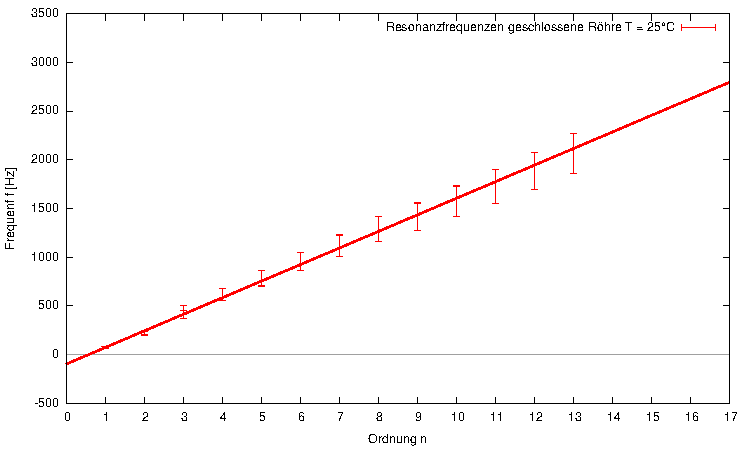
\includegraphics[width=\textwidth]{graphen/gnuplot/a2_1}}
\captionof{figure}{Messung der geschlossenen Röhre}
\end{minipage}

\begin{minipage}{\linewidth}
\centering
\makebox[0cm]{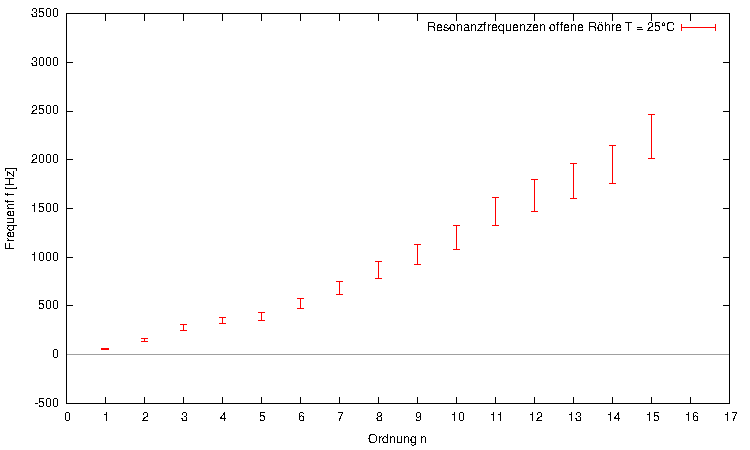
\includegraphics[width=\textwidth]{graphen/gnuplot/a2_2}}
\captionof{figure}{Messung der offenen Röhre}
\end{minipage}
\end{center}
\newpage
\subsection{Auswertung}
\subsubsection{geschlossene Röhre}
Wie zu sehen ist liefert die Messung des geschlossenen Rohrs einen sehr linearen Verlauf und der Verlauf kann mit einer Kurve \(f(x)=a+b \cdot x\) approximiert werden. Über eine gewichtete lineare Regression wurden so die Parameter \(a\) und \(b\) bestimmt.

\begin{center}
\noindent
\begin{minipage}{\linewidth}
\centering
\makebox[0cm]{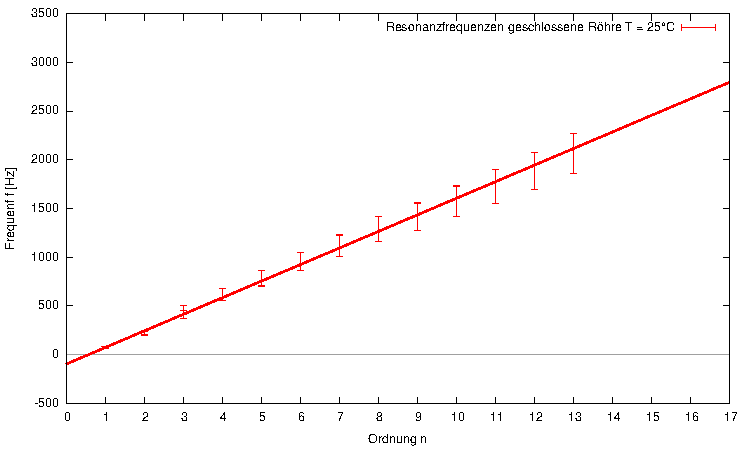
\includegraphics[width=\textwidth]{graphen/gnuplot/a2_1'}}
\captionof{figure}{Messung der geschlossenen Röhre}
\end{minipage}
\end{center}

\begin{align}
a_g &= \left( -97,2 \pm 3,2 \right)\, Hz \notag \\ 
b_g &= \left( 170,2 \pm 1,8 \right)\, Hz \notag
\end{align}

\subsubsection{offene Röhre}
Die Messung mit offenem Rohrende dagegen lieferte keinen linearen Verlauf, was auch daran liegen könnte, dass diese aufgrund von Zeitmangel nicht wiederholt werden konnte, und somit keine Vergleichswerte vorhanden sind. Um die Daten dennoch auswerten zu können werden die Messwerte, die nicht in den Verlauf passen gestrichen und man erhält eine modifizierte Wertetabelle:
\begin{center}
\begin{tabular}{c|c}
Ordnung \(n\) & Resonanzfrequnzen \(f\) \\\hline
\(1\) & \( 153\) \\ 
\(2\) & \( 350\) \\ 
\(3\) & \( 528\) \\ 
\(4\) & \( 683\) \\ 
\(5\) & \( 866\) \\ 
\(6\) & \( 1030\) \\ 
\(07\) & \( 1205\) \\ 
\(09\) & \( 1471\) \\ 
\(10\) & \( 1636\) \\ 
\(11\) & \( 1784\) \\ 
\(12\) & \( 1955\) \\ 
\(13\) & \( 2243\) \\
\end{tabular}
\end{center}
Nun liefern auch diese Daten mit linearer Regression eine Sinnvolle Gerade:

\begin{center}
\noindent
\begin{minipage}{\linewidth}
\centering
\makebox[0cm]{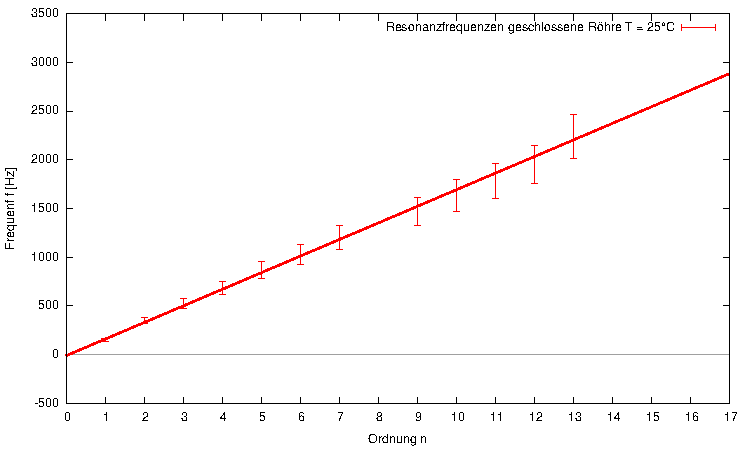
\includegraphics[width=\textwidth]{graphen/gnuplot/a2_2'}}
\captionof{figure}{Messung der geschlossenen Röhre}
\end{minipage}
\end{center}
Mit den Parametern:
\begin{align}
a_o &= \left( -10,9 \pm 7,1 \right)\, Hz \notag \\ 
b_o &= \left( 170,4 \pm 2,7 \right)\, Hz \notag
\end{align}
\captionof{table}{Modifizierte Messwerte der Messung mit offenem Rohr}
\subsubsection{Ermitteln der Schallgeschwindigkeit}
Zusammenfassend sind somit folgende Parameter ermittelt worden:
\begin{align}
a_g &= \left( -97,2 \pm 3,2 \right)\, Hz \notag \\ 
b_g &= \left( 170,2 \pm 1,8 \right)\, Hz \notag \\
a_o &= \left( -10,9 \pm 7,1 \right)\, Hz \notag \\ 
b_o &= \left( 170,4 \pm 2,7 \right)\, Hz \notag
\end{align}
Die Gleichungen \eqref{geschlossen} und \eqref{offen} liefern mit \(\lambda = \frac{c}{f}\) Funktionen \(f(n)\):
\begin{align}
f_1(n) &= n \cdot \frac{c}{2l} \\
f_2(n) &= n \cdot \frac{c}{2l} - \frac{c}{4l}
\end{align}
Der Ordinatenabschnitt  \(a\) verschwindet also im Falle zweier offener oder geschlossener Enden. Da der Ordinatenabschnitt im Falle des offenen Endes viel kleiner ist wird der Lautsprecher als offenes Ende interpretiert.
Die Steigungen \(b\) können jeweils identifiziert werden als:
\begin{align}
b &= \frac{c}{2l}\\
\Rightarrow c &= 2l \cdot b \\
\Delta c &= c\cdot \sqrt{\left( \frac{\Delta l}{l} \right)^2+\left( \frac{\Delta b}{b} \right)^2} \\
c_o &= \left(346,9 \pm 5,6 \right)\, \frac{m}{s} \notag \\
c_g &= \left(346,5 \pm 3,8 \right)\, \frac{m}{s} \notag
\end{align}

Da beide Kurven auch systematische Fehler enthalten kann der Wert von \(a_0\) als solcher interpretiert werden. Da angenommen wird, dass das Ende mit Lautsprecher offen ist, kann man  systematische Fehler \(a_o\) von \(a_g\) subtrahieren und erhält:
\begin{align}
a_g' &= a_g - a_o = -86,3\, Hz \notag \\
\Delta a_g' &= \sqrt{\left(\Delta a_o\right)^2 + \left(\Delta a_g\right)^2} = 7,8\, Hz \notag
\end{align}
Das passt perfekt zum theoretischen Ordinatenabschnitt \(-\frac{c}{4l} \approx - 85\, Hz\).

Um aus den Schallgeschwindigkeiten nun den Isentropenindex \(\kappa\) zu bestimmen wird Gleichung \eqref{c(T)} umgestellt zu:
\begin{align}
\kappa &= c^2 \cdot \frac{M}{RT} \\
\Rightarrow \Delta \kappa &= \kappa \cdot \sqrt{\left(\frac{2\Delta c}{c}\right)^2+ \left(\frac{\Delta T}{T}\right)^2}
\end{align} 
Leider wurde versäumt die Temperatur zu Messen, da es ein warmer Sommertag wird \(T\) auf \((25 \pm 3)\,^\circ C = (198,15 \pm 3)\, K\) geschätzt. Für die Schallgeschwindigkeit wird der genauere Wert von \(c_g = (346,5 \pm 3,8)\, \frac{m}{s}\) verwendet, \(R = 8,314\, \frac{J}{mol\cdot K}\) ist die universelle Gaskonstante, \(M = 0,02896\, \frac{kg}{mol}\) ist die molare Masse von Luft.
\begin{align}
\kappa =  1,403 \pm 0,034 \notag
\end{align} 

\subsection{Fazit und Vergleich}
Der versuch war sehr gut durchführbar und lieferte sehr genaue Ergebnisse. Da bei der offenen Röhre die Werte keinen linearen Verlauf annehmen und eine Modifikation der Messwerte notwendig war ist der Wert für \(c_o\) nur konstruiert und sollte nochmals überprüft werden. Zusammengefasst wurden somit folgende Werte ermittelt:
\begin{align}
c_o &= \left(347 \pm 6 \right)\, \frac{m}{s} \notag \\
c_g &= \left(346 \pm 4 \right)\, \frac{m}{s} \notag \\
\kappa &= 1,40 \pm 0,04 \notag
\end{align}
Diese sind alle identisch zu den Literaturwerten da die einfachen Fehlerintervalle die Literaturwerte umschließen. Diese sind \(c \approx 343\, \frac{m}{s}\) bzw. \(\kappa \approx 1,402\). 

